% Options for packages loaded elsewhere
\PassOptionsToPackage{unicode}{hyperref}
\PassOptionsToPackage{hyphens}{url}
%
\documentclass[
]{article}
\usepackage{lmodern}
\usepackage{stata}
\usepackage{amssymb,amsmath}
\usepackage{ifxetex,ifluatex}
\ifnum 0\ifxetex 1\fi\ifluatex 1\fi=0 % if pdftex
  \usepackage[T1]{fontenc}
  \usepackage[utf8]{inputenc}
  \usepackage{textcomp} % provide euro and other symbols
\else % if luatex or xetex
  \usepackage{unicode-math}
  \defaultfontfeatures{Scale=MatchLowercase}
  \defaultfontfeatures[\rmfamily]{Ligatures=TeX,Scale=1}
\fi
% Use upquote if available, for straight quotes in verbatim environments
\IfFileExists{upquote.sty}{\usepackage{upquote}}{}
\IfFileExists{microtype.sty}{% use microtype if available
  \usepackage[]{microtype}
  \UseMicrotypeSet[protrusion]{basicmath} % disable protrusion for tt fonts
}{}
\makeatletter
\@ifundefined{KOMAClassName}{% if non-KOMA class
  \IfFileExists{parskip.sty}{%
    \usepackage{parskip}
  }{% else
    \setlength{\parindent}{0pt}
    \setlength{\parskip}{6pt plus 2pt minus 1pt}}
}{% if KOMA class
  \KOMAoptions{parskip=half}}
\makeatother
\usepackage{xcolor}
\IfFileExists{xurl.sty}{\usepackage{xurl}}{} % add URL line breaks if available
\IfFileExists{bookmark.sty}{\usepackage{bookmark}}{\usepackage{hyperref}}
\hypersetup{
  pdftitle={Multiple Approaches to Causal Modeling Using Black Spruce Data},
  pdfauthor={Andy Grogan-Kaylor},
  hidelinks,
  pdfcreator={LaTeX via pandoc}}
\urlstyle{same} % disable monospaced font for URLs
\usepackage{graphicx,grffile}
\makeatletter
\def\maxwidth{\ifdim\Gin@nat@width>\linewidth\linewidth\else\Gin@nat@width\fi}
\def\maxheight{\ifdim\Gin@nat@height>\textheight\textheight\else\Gin@nat@height\fi}
\makeatother
% Scale images if necessary, so that they will not overflow the page
% margins by default, and it is still possible to overwrite the defaults
% using explicit options in \includegraphics[width, height, ...]{}
\setkeys{Gin}{width=\maxwidth,height=\maxheight,keepaspectratio}
% Set default figure placement to htbp
\makeatletter
\def\fps@figure{htbp}
\makeatother
\setlength{\emergencystretch}{3em} % prevent overfull lines
\providecommand{\tightlist}{%
  \setlength{\itemsep}{0pt}\setlength{\parskip}{0pt}}
\setcounter{secnumdepth}{-\maxdimen} % remove section numbering

\title{Multiple Approaches to Causal Modeling Using Black Spruce Data}
\author{Andy Grogan-Kaylor}
\date{12 Apr 2021 15:44:55}

\begin{document}
\maketitle

\hypertarget{background}{%
\section{Background 🌲}\label{background}}

\begin{quote}
In web slide versions of this material press \texttt{b} for bigger text
and \texttt{s} for smaller text.
\end{quote}

Chihara and Hesterberg (2018) provide a data set concerning the growth
of Black Spruce Trees. According to these authors:

\begin{quote}
``Black spruce (Picea mariana) is a species of a slow-growing coniferous
tree found across the northern part of North America. It is commonly
found on wet organic soils. In a study conducted in the 1990s, a
biologist interested in factors affecting the growth of the black spruce
planted its seedlings on sites located in boreal peatlands in northern
Manitoba, Canada (Camil et al.~(2010)). The data set Spruce contains a
part of the data from the study (Table 1.8). Seventy-two black spruce
seedlings were planted in four plots under varying conditions
(fertilizer--no fertilizer, competition--no competition), and their
heights and diameters were measured over the course of 5 years. The
researcher wanted to see whether the addition of fertilizer or the
removal of competition from other plants (by weeding) affected the
growth of these seedlings.''
\end{quote}

\hypertarget{the-research-question}{%
\section{The Research Question 🌲}\label{the-research-question}}

\begin{quote}
We are going to consider the \emph{potentially causal} estimate of the
effect of \emph{fertilizer} on \emph{tree height at year 5}. Along the
way we will give brief attention to the advantages and disadvantages of
each approach. Because of the research design, we have strong reasons to
consider \emph{fertilizer} as having a causal effect on \emph{tree
height} but we will nonetheless explore this question using a variety of
statistical models.
\end{quote}

\begin{quote}
A secondary purpose of this document is to demonstrate that Stata syntax
makes it easy to test and compare multiple statistical models because of
the uniform Stata syntax, which is almost always:
\texttt{command\ variable(s),\ options}.
\end{quote}

\hypertarget{causality}{%
\section{Causality 🌲}\label{causality}}

\includegraphics[width=0.25\textwidth,height=\textheight]{causality.png}

A variable \(x\) can only be considered to have \emph{causal}
association with \(y\) if the following conditions are met (Holland,
1986):

\begin{enumerate}
\def\labelenumi{\arabic{enumi}.}
\tightlist
\item
  \(x\) is correlated with \(y\).
\item
  \(x\) precedes \(y\) in time order.
\item
  The association between \(x\) and \(y\) can not be accounted for by
  any third variable \(z\).
\end{enumerate}

Hence, for this particular data, we are exploring:

\includegraphics[width=0.25\textwidth,height=\textheight]{spruce.png}

\begin{quote}
What happens to the association of \emph{fertilizer} and \emph{tree
height} when we control for possible confounding variables \(z\) using
various statistical strategies?
\end{quote}

(For more interactive exploration of these ideas, see
\href{https://agrogan.shinyapps.io/causality/?_inputs_\&sidebarCollapsed=false\&y=\%22tree\%20height\%22\&sidebarItemExpanded=null\&x=\%22fertilizer\%22\&z=\%22alternative\%20explanation\%22}{this
demo}).

\hypertarget{setup}{%
\section{Setup 🌲}\label{setup}}

\hypertarget{get-data}{%
\subsection{Get Data}\label{get-data}}

\begin{stlog}
. clear all
{\smallskip}
.         
. use spruce.dta, clear
\end{stlog}

\hypertarget{dataset-description}{%
\subsection{Dataset Description}\label{dataset-description}}



\begin{stlog}
. describe    
{\smallskip}
Contains data from spruce.dta
  obs:            72                          
 vars:             9                          26 Apr 2020 12:18
\HLI{84}
              storage   display    value
variable name   type    format     label      variable label
\HLI{84}
Tree            long    \%12.0g                Tree number
Competition     long    \%12.0g     Competition
                                              C (competition), CR (competition
                                                removed)
Fertilizer      long    \%12.0g     Fertilizer
                                              F (fertilized), NF (not fertilized)
Height0         double  \%10.0g                Height (cm) of seedling at planting
Height5         double  \%10.0g                Height (cm) of seedling at year 5
Diameter0       double  \%10.0g                Diameter (cm) of seedling at planting
Diameter5       double  \%10.0g                Diameter (cm) of seedling at year 5
Ht_change       double  \%10.0g                Change (cm) in height
Di_change       double  \%10.0g                Change (cm) in diameter
\HLI{84}
Sorted by: 
\end{stlog}

\hypertarget{spruce-data-and-causal-criteria}{%
\section{Spruce Data And Causal Criteria
🌲}\label{spruce-data-and-causal-criteria}}

Let's consider in turn each of the criteria for causality.

\begin{enumerate}
\def\labelenumi{\arabic{enumi}.}
\tightlist
\item
  Empirically, \emph{fertilizer} is correlated with \emph{tree height}.
\end{enumerate}



\begin{figure}
\centering
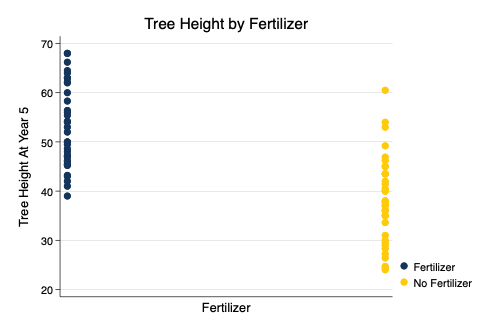
\includegraphics[width=0.25\textwidth,height=\textheight]{myscatter.png}
\caption{Scatterplot of Tree Height At Year 5 By Fertilizer Use}
\end{figure}

\begin{enumerate}
\def\labelenumi{\arabic{enumi}.}
\setcounter{enumi}{1}
\tightlist
\item
  From the research design, we know that \emph{fertilizer} comes prior
  to \emph{tree height at year 5}.
\item
  We are going to use various statistical strategies--detailed below--to
  assess whether the association of \emph{fertilizer} and \emph{tree
  height} can be accounted for by any third variable.
\end{enumerate}

\hypertarget{analyses}{%
\section{Analyses 🌲}\label{analyses}}

\hypertarget{t-test}{%
\subsection{t Test}\label{t-test}}

A t test compares the difference between the means of two groups to the
standard error of the difference between means.

Formally, \(t = \frac{\bar{x}_2 - \bar{x}_1}{s}\) where s is the
standard error of the estimate of the mean.

More colloquially, the t test compares the differences between the two
groups in standard error units.

A t test does \emph{not} control for any additional variable(s).

\begin{stlog}
. ttest Height5, by(Fertilizer)
{\smallskip}
Two-sample t test with equal variances
\HLI{9}{\TOPT}\HLI{68}
Variable {\VBAR}     Obs        Mean    Std. Err.   Std. Dev.   [95\% Conf. Interval]
\HLI{9}{\PLUS}\HLI{68}
       F {\VBAR}      36    52.89167    1.396079    8.376476    50.05747    55.72586
      NF {\VBAR}      36    38.11944    1.465226    8.791354    35.14488    41.09401
\HLI{9}{\PLUS}\HLI{68}
combined {\VBAR}      72    45.50556    1.333392    11.31421    42.84685    48.16426
\HLI{9}{\PLUS}\HLI{68}
    diff {\VBAR}            14.77222    2.023839                 10.7358    18.80864
\HLI{9}{\BOTT}\HLI{68}
    diff = mean(F) - mean(NF)                                     t =   7.2991
Ho: diff = 0                                     degrees of freedom =       70
{\smallskip}
    Ha: diff < 0                 Ha: diff != 0                 Ha: diff > 0
 Pr(T < t) = 1.0000         Pr(|T| > |t|) = 0.0000          Pr(T > t) = 0.0000
\end{stlog}

\begin{quote}
The association of fertilizer with tree height is -14.77.
\end{quote}

\hypertarget{ols-regression}{%
\subsection{OLS Regression}\label{ols-regression}}

A regression estimates the association of a 1 unit change in each of the
independent variables with change in the dependent variable, while
accounting for all of the other independent variables in the model.

\(y_i = \beta_0 + \beta_1 x_{1i} + \Sigma \beta_k x_{ki} + e_i\)

Here \(x_{1i}\) is the treatment variable of interest.

A regression controls for the additional observed variables (\(x_{ki}\))
that are included in the model.

\begin{stlog}
. regress Height5 Fertilizer Height0 Competition
{\smallskip}
      Source {\VBAR}       SS           df       MS      Number of obs   =        72
\HLI{13}{\PLUS}\HLI{34}   F(3, 68)        =     50.97
       Model {\VBAR}  6291.23189         3   2097.0773   Prob > F        =    0.0000
    Residual {\VBAR}  2797.56589        68  41.1406748   R-squared       =    0.6922
\HLI{13}{\PLUS}\HLI{34}   Adj R-squared   =    0.6786
       Total {\VBAR}  9088.79778        71  128.011236   Root MSE        =    6.4141
{\smallskip}
\HLI{13}{\TOPT}\HLI{64}
     Height5 {\VBAR}      Coef.   Std. Err.      t    P>|t|     [95\% Conf. Interval]
\HLI{13}{\PLUS}\HLI{64}
  Fertilizer {\VBAR}  -14.71947   1.511991    -9.74   0.000    -17.73661   -11.70234
     Height0 {\VBAR}   .8631456    .374817     2.30   0.024       .11521    1.611081
 Competition {\VBAR}   10.52346    1.52143     6.92   0.000      7.48749    13.55942
       _cons {\VBAR}   39.22163   6.189971     6.34   0.000     26.86974    51.57353
\HLI{13}{\BOTT}\HLI{64}
\end{stlog}

\begin{quote}
The association of fertilizer with tree height is -14.72.
\end{quote}

\hypertarget{propensity-scores}{%
\subsection{Propensity Scores}\label{propensity-scores}}

The propensity score estimates the probability of being administered the
treatment, in this example, \emph{fertilizer}. Treatment observations
are matched to the most similar comparison group observation in terms of
this probability, and an average difference is calculated.

A propensity score analysis controls for the additional observed
variables that are included in the model.

\begin{stlog}
. teffects psmatch (Height5) (Fertilizer Height0 Competition)
{\smallskip}
Treatment-effects estimation                   Number of obs      =         72
Estimator      : propensity-score matching     Matches: requested =          1
Outcome model  : matching                                     min =          1
Treatment model: logit                                        max =          3
\HLI{13}{\TOPT}\HLI{64}
             {\VBAR}              AI Robust
     Height5 {\VBAR}      Coef.   Std. Err.      z    P>|z|     [95\% Conf. Interval]
\HLI{13}{\PLUS}\HLI{64}
ATE          {\VBAR}
  Fertilizer {\VBAR}
  (NF vs F)  {\VBAR}  -12.71019   1.988531    -6.39   0.000    -16.60763   -8.812737
\HLI{13}{\BOTT}\HLI{64}
\end{stlog}



\begin{quote}
The association of fertilizer with tree height is -12.71.
\end{quote}

\hypertarget{assess-balance-of-propensity-score-model-cuartas}{%
\subsubsection[Assess Balance of Propensity Score Model
]{\texorpdfstring{Assess Balance of Propensity Score Model \footnote{With
  many thanks to Jorge Cuartas for ideas for some of this code.}}{Assess Balance of Propensity Score Model }}\label{assess-balance-of-propensity-score-model-cuartas}}

\begin{stlog}
. tebalance density, ///
> scheme(michigan)
note: refitting the model using the {\bftt{generate()}} option
{\smallskip}
. 
. graph export mydensity.png, width(500) replace
(file /Users/agrogan/Desktop/newstuff/spruce/mydensity.png written in PNG format)
\end{stlog}



\begin{figure}
\centering
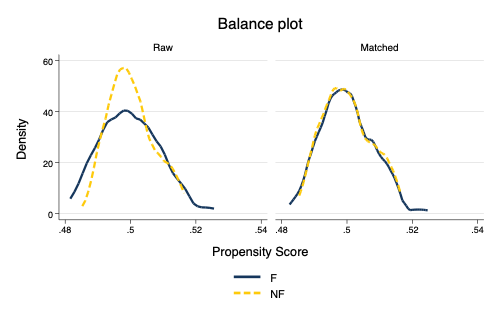
\includegraphics[width=0.75\linewidth]{mydensity.png}
\caption{Density Plot of Propensity Score}
\end{figure}



\hypertarget{references}{%
\section{References 🌲}\label{references}}

Camill, P., Chihara, L., Adams, B., Andreassi, C., Barry, A. N. N.,
Kalim, S., \ldots{} Rafert, G. (2010). Early life history transitions
and recruitment of Picea mariana in thawed boreal permafrost peatlands.
\emph{Ecology}. https://doi.org/10.1890/08-1839.1

Chihara, L. M., \& Hesterberg, T. C. (2018). \emph{Mathematical
Statistics with Resampling and R}. https://doi.org/10.1002/9781119505969

Holland, P. W. (1986). Statistics and Causal Inference. \emph{Journal of
the American Statistical Association}, 81(396), 945--960.
https://doi.org/10.1080/01621459.1986.10478354

\end{document}
